\section*{Введение}

В данной лабораторной работе рассматривается связь между непрерывным и дискретным преобразованием Фурье, а также исследуется теорема Найквиста-Шеннона-Котельникова. Эти концепции являются фундаментальными для понимания цифровой обработки сигналов.

\textbf{Цель работы:} изучение различных методов вычисления преобразования Фурье и исследование теоремы сэмплирования на практических примерах.

\textbf{Задачи:}
\begin{enumerate}
    \item Сравнение различных методов вычисления преобразования Фурье
    \item Исследование точности и быстродействия численного интегрирования и DFT
    \item Разработка методов получения точного непрерывного преобразования с помощью DFT
    \item Исследование теоремы Найквиста-Шеннона-Котельникова на примерах
\end{enumerate}

\section*{Задание 1. Непрерывное и дискретное преобразование Фурье}

\subsection*{Постановка задачи}

Рассматривается прямоугольная функция $\Pi: \mathbb{R} \to \mathbb{R}$:
\begin{equation}
\Pi(t) = \begin{cases}
1, & |t| \leq 1/2 \\
0, & |t| > 1/2
\end{cases}
\end{equation}

Требуется сравнить различные методы вычисления преобразования Фурье:
\begin{itemize}
    \item Аналитическое вычисление истинного Фурье-образа
    \item Численное интегрирование с помощью функции trapz
    \item Дискретное преобразование Фурье (DFT)
    \item Умное использование DFT для получения точного непрерывного преобразования
\end{itemize}

\subsection*{Истинный Фурье-образ}

Аналитическое выражение для Фурье-образа прямоугольной функции:
\begin{equation}
\hat{\Pi}(\nu) = \int_{-\infty}^{+\infty} \Pi(t) e^{-2\pi i \nu t} dt = \int_{-1/2}^{1/2} e^{-2\pi i \nu t} dt
\end{equation}

Вычисляя интеграл:
\begin{equation}
\hat{\Pi}(\nu) = \frac{e^{-2\pi i \nu t}}{-2\pi i \nu} \Bigg|_{-1/2}^{1/2} = \frac{e^{-\pi i \nu} - e^{\pi i \nu}}{-2\pi i \nu} = \frac{\sin(\pi \nu)}{\pi \nu} = \text{sinc}(\nu)
\end{equation}

Таким образом, Фурье-образ прямоугольной функции есть функция sinc:
\begin{equation}
\hat{\Pi}(\nu) = \text{sinc}(\nu) = \frac{\sin(\pi \nu)}{\pi \nu}
\end{equation}

\begin{figure}[H]
    \centering
    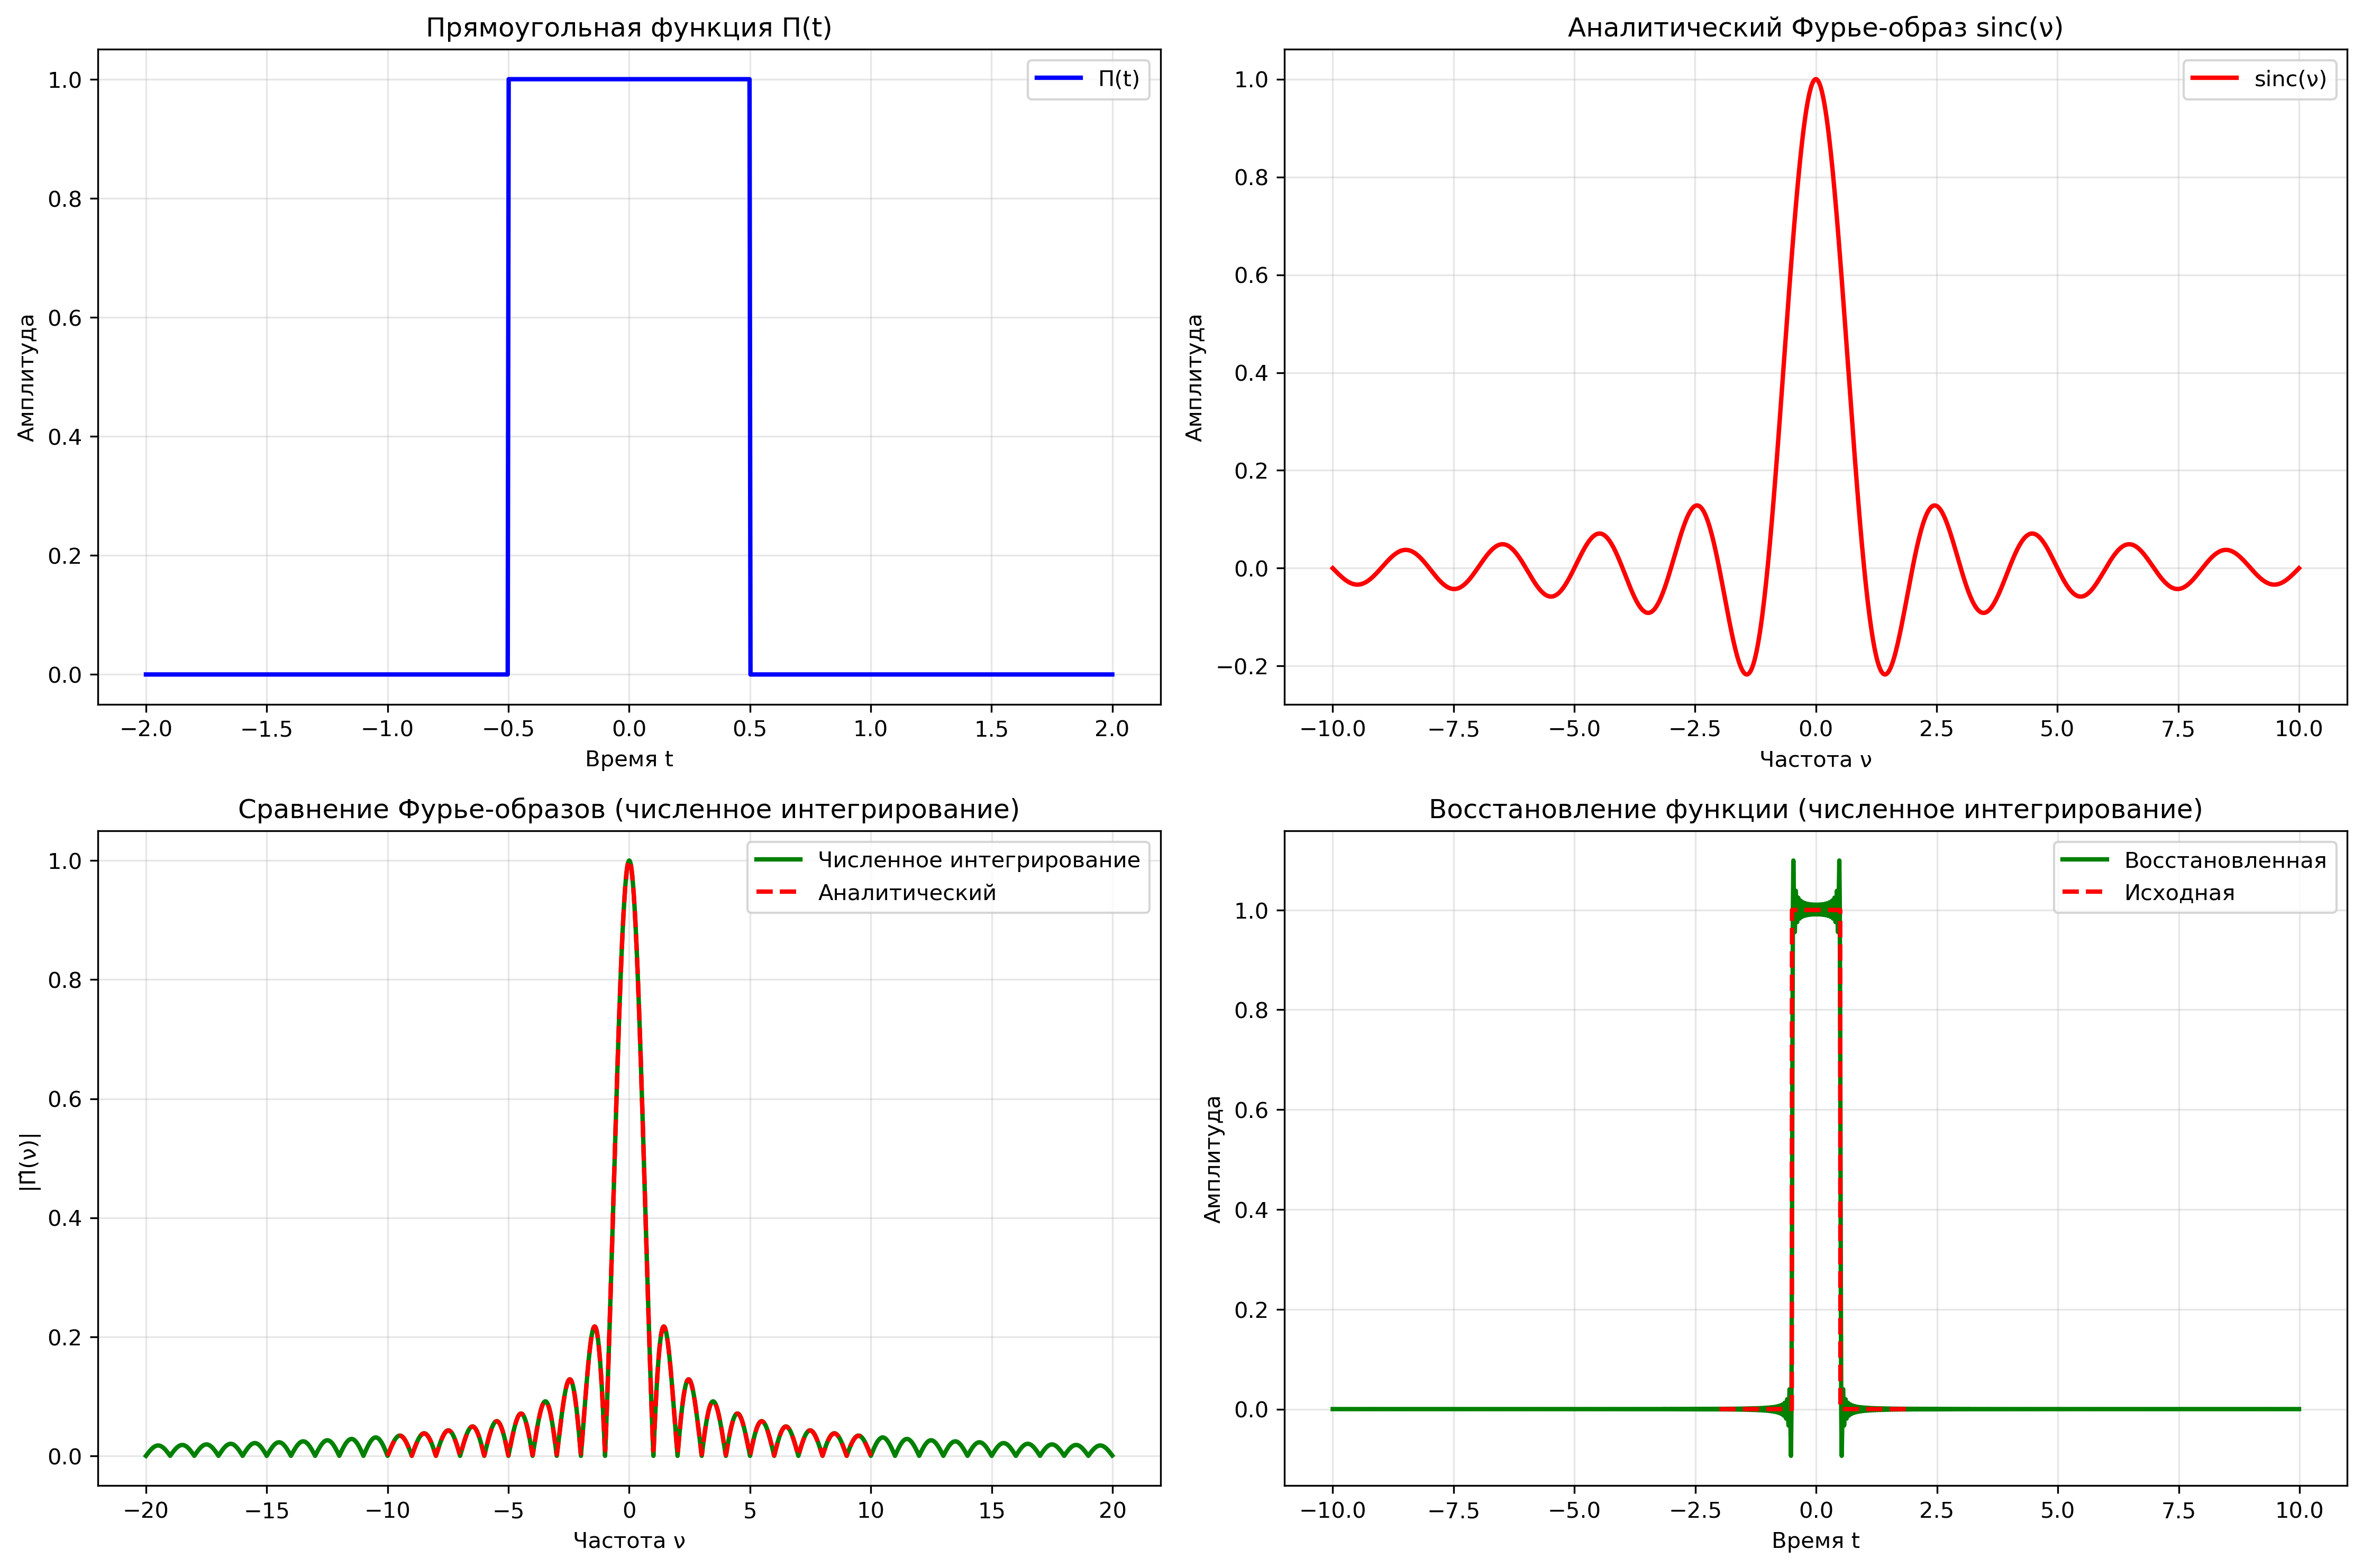
\includegraphics[width=0.8\textwidth]{images/task1/analytical_and_trapz_comparison.png}
    \caption{Сравнение аналитического и численного методов}
    \label{fig:analytical_trapz}
\end{figure}

\begin{figure}[H]
    \centering
    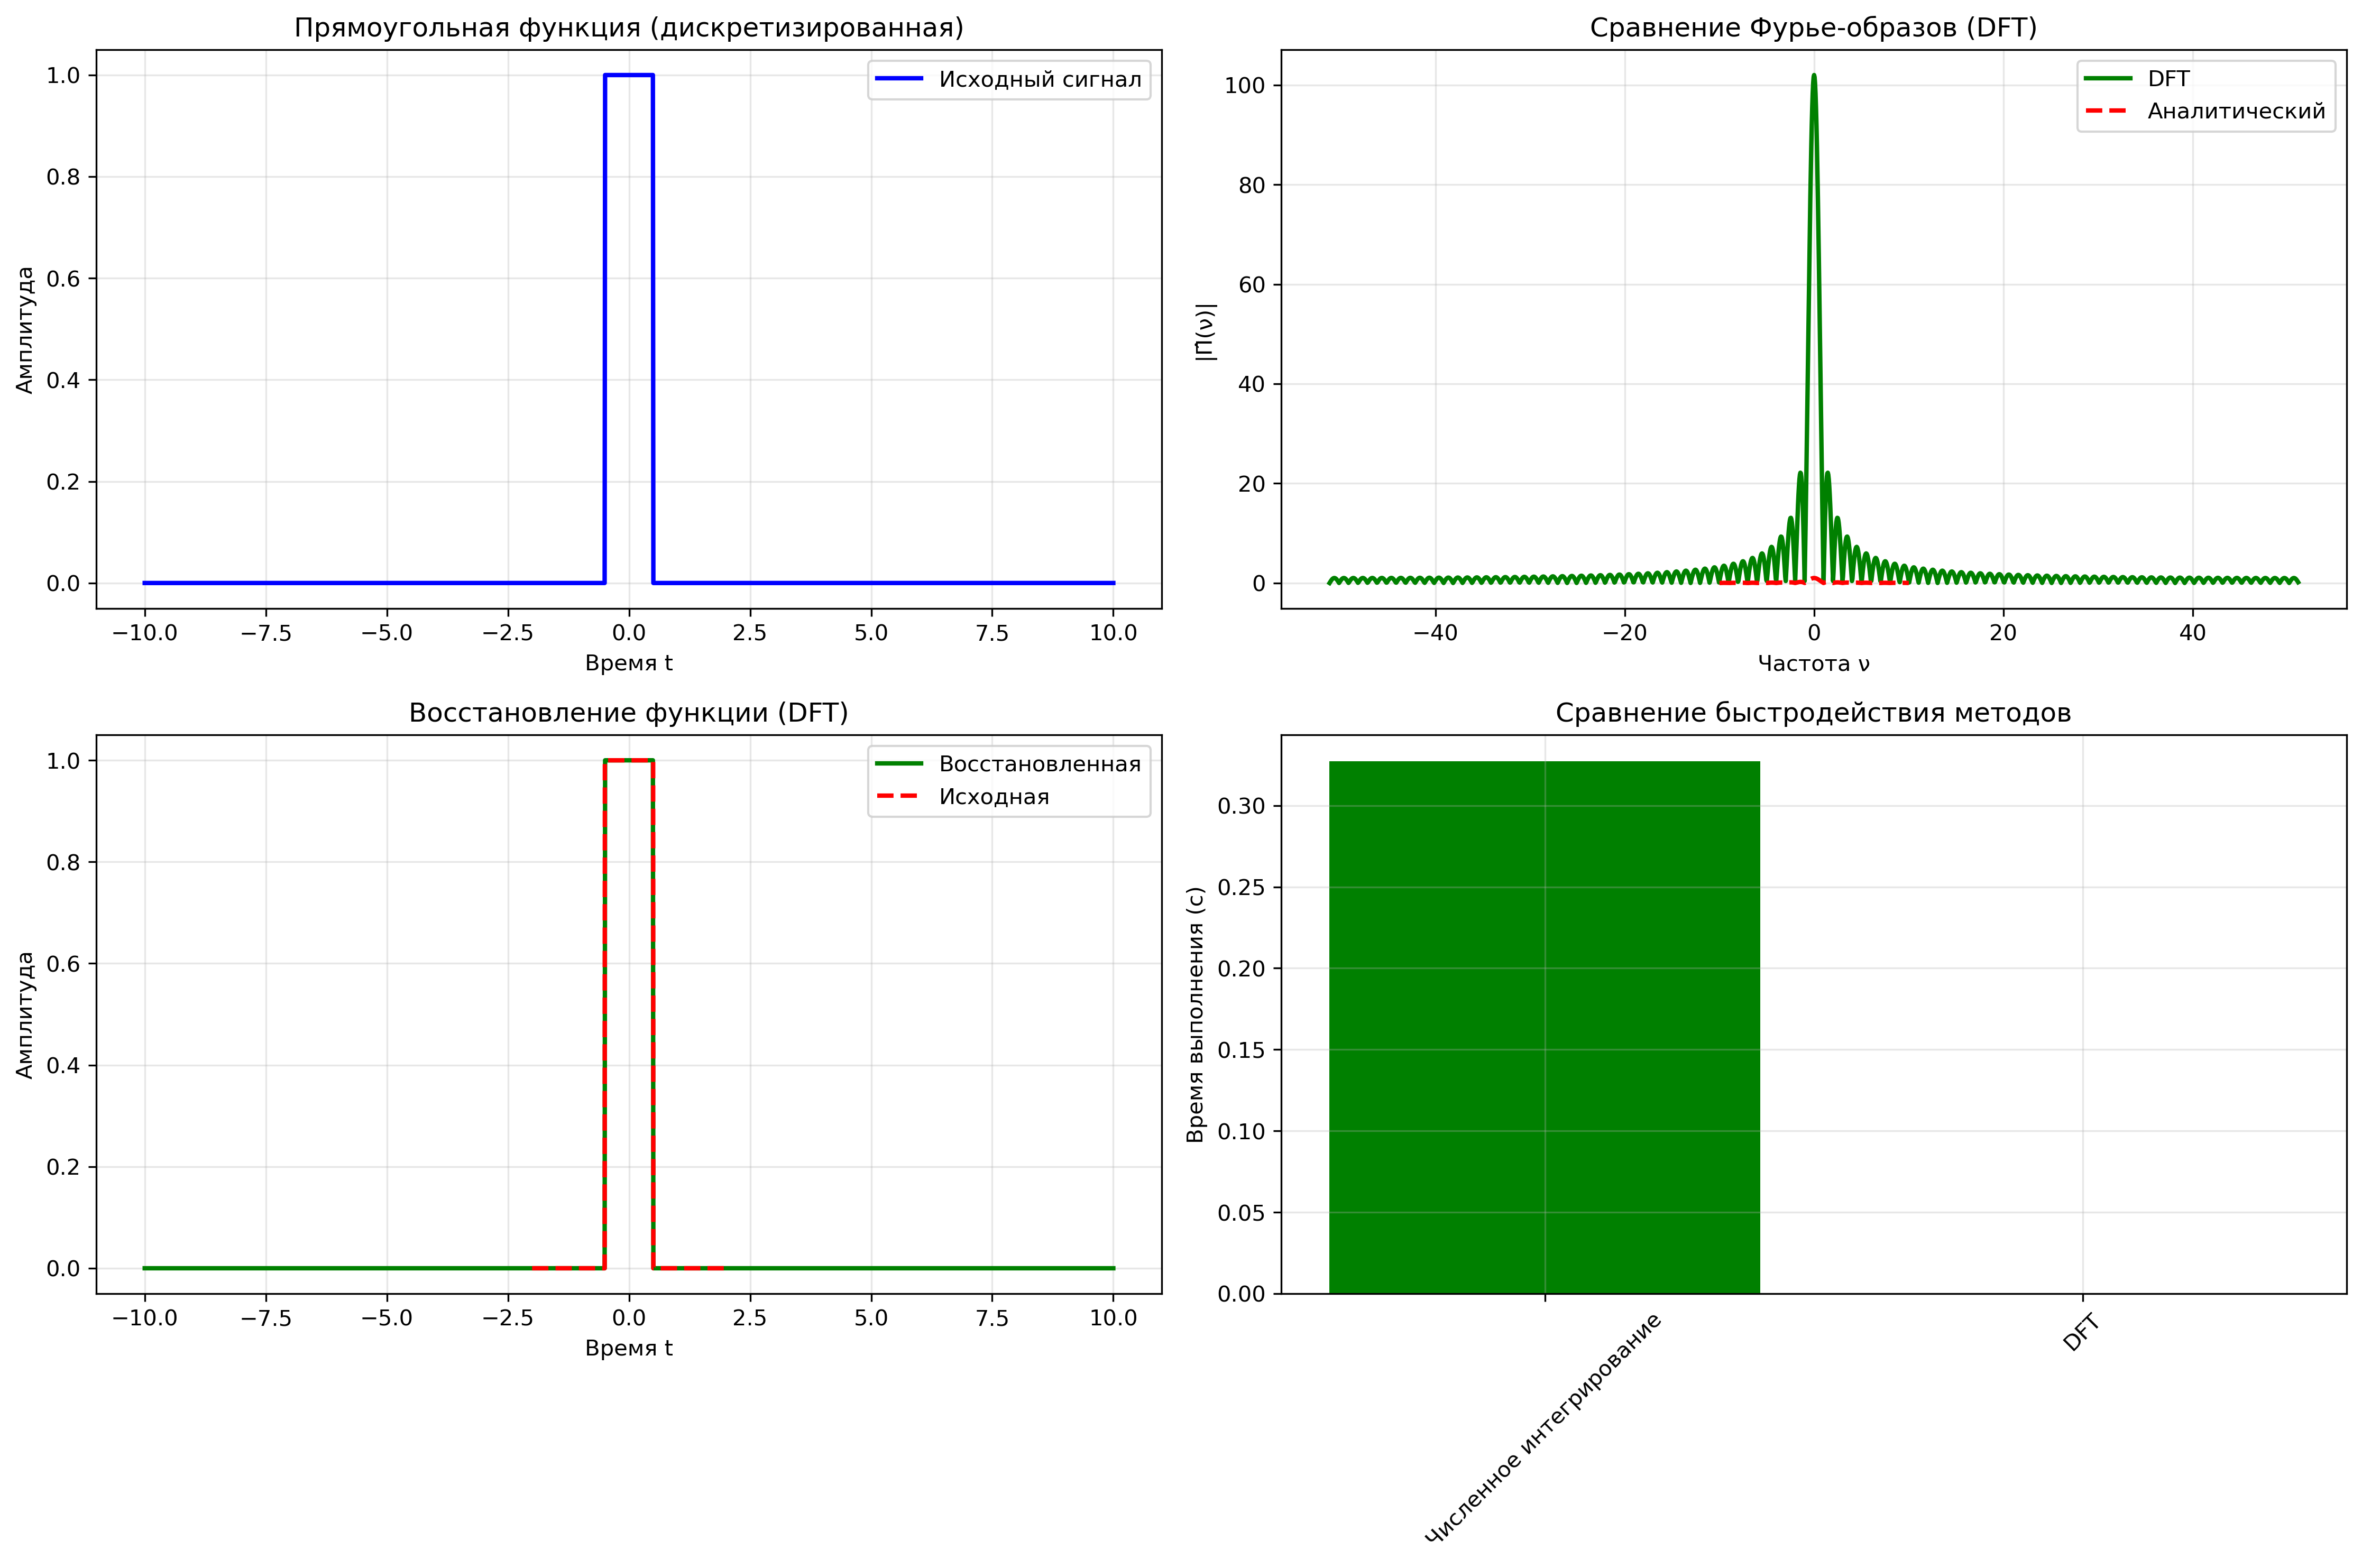
\includegraphics[width=0.8\textwidth]{images/task1/dft_comparison.png}
    \caption{Сравнение DFT метода с аналитическим решением}
    \label{fig:dft_comparison}
\end{figure}

\begin{figure}[H]
    \centering
    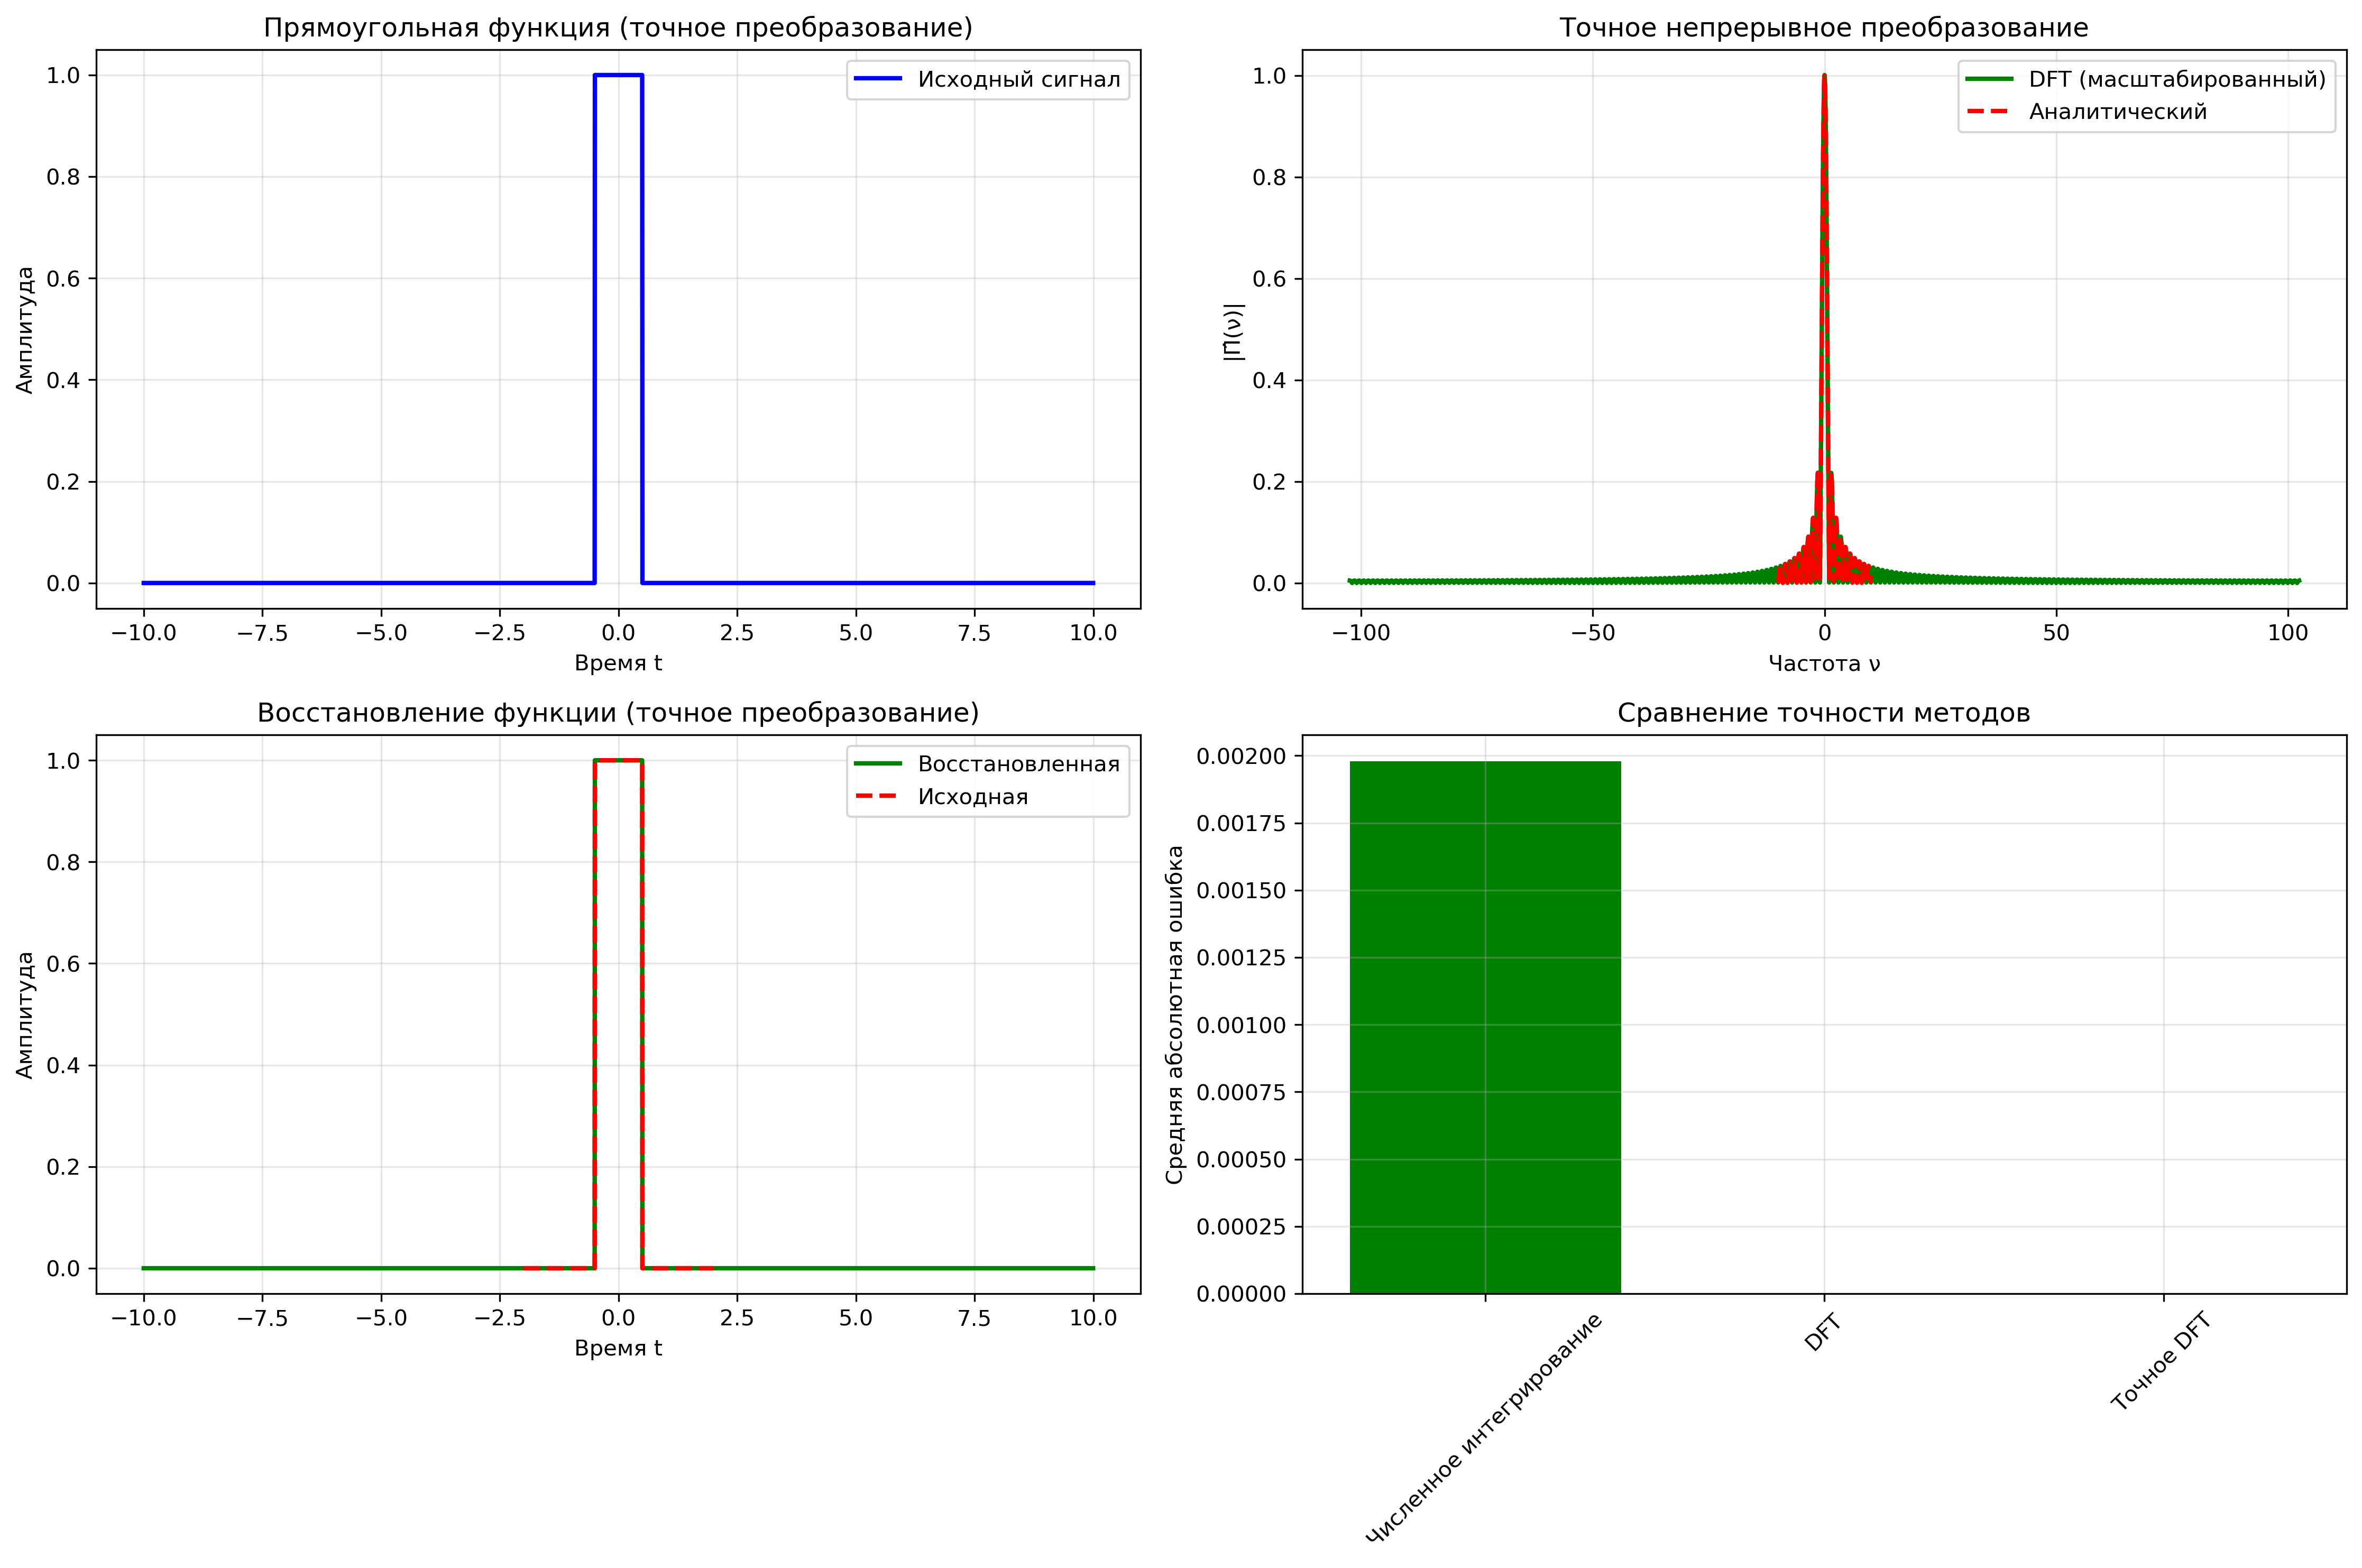
\includegraphics[width=0.8\textwidth]{images/task1/precise_fourier_comparison.png}
    \caption{Точное непрерывное преобразование с помощью DFT}
    \label{fig:precise_fourier}
\end{figure}

\begin{figure}[H]
    \centering
    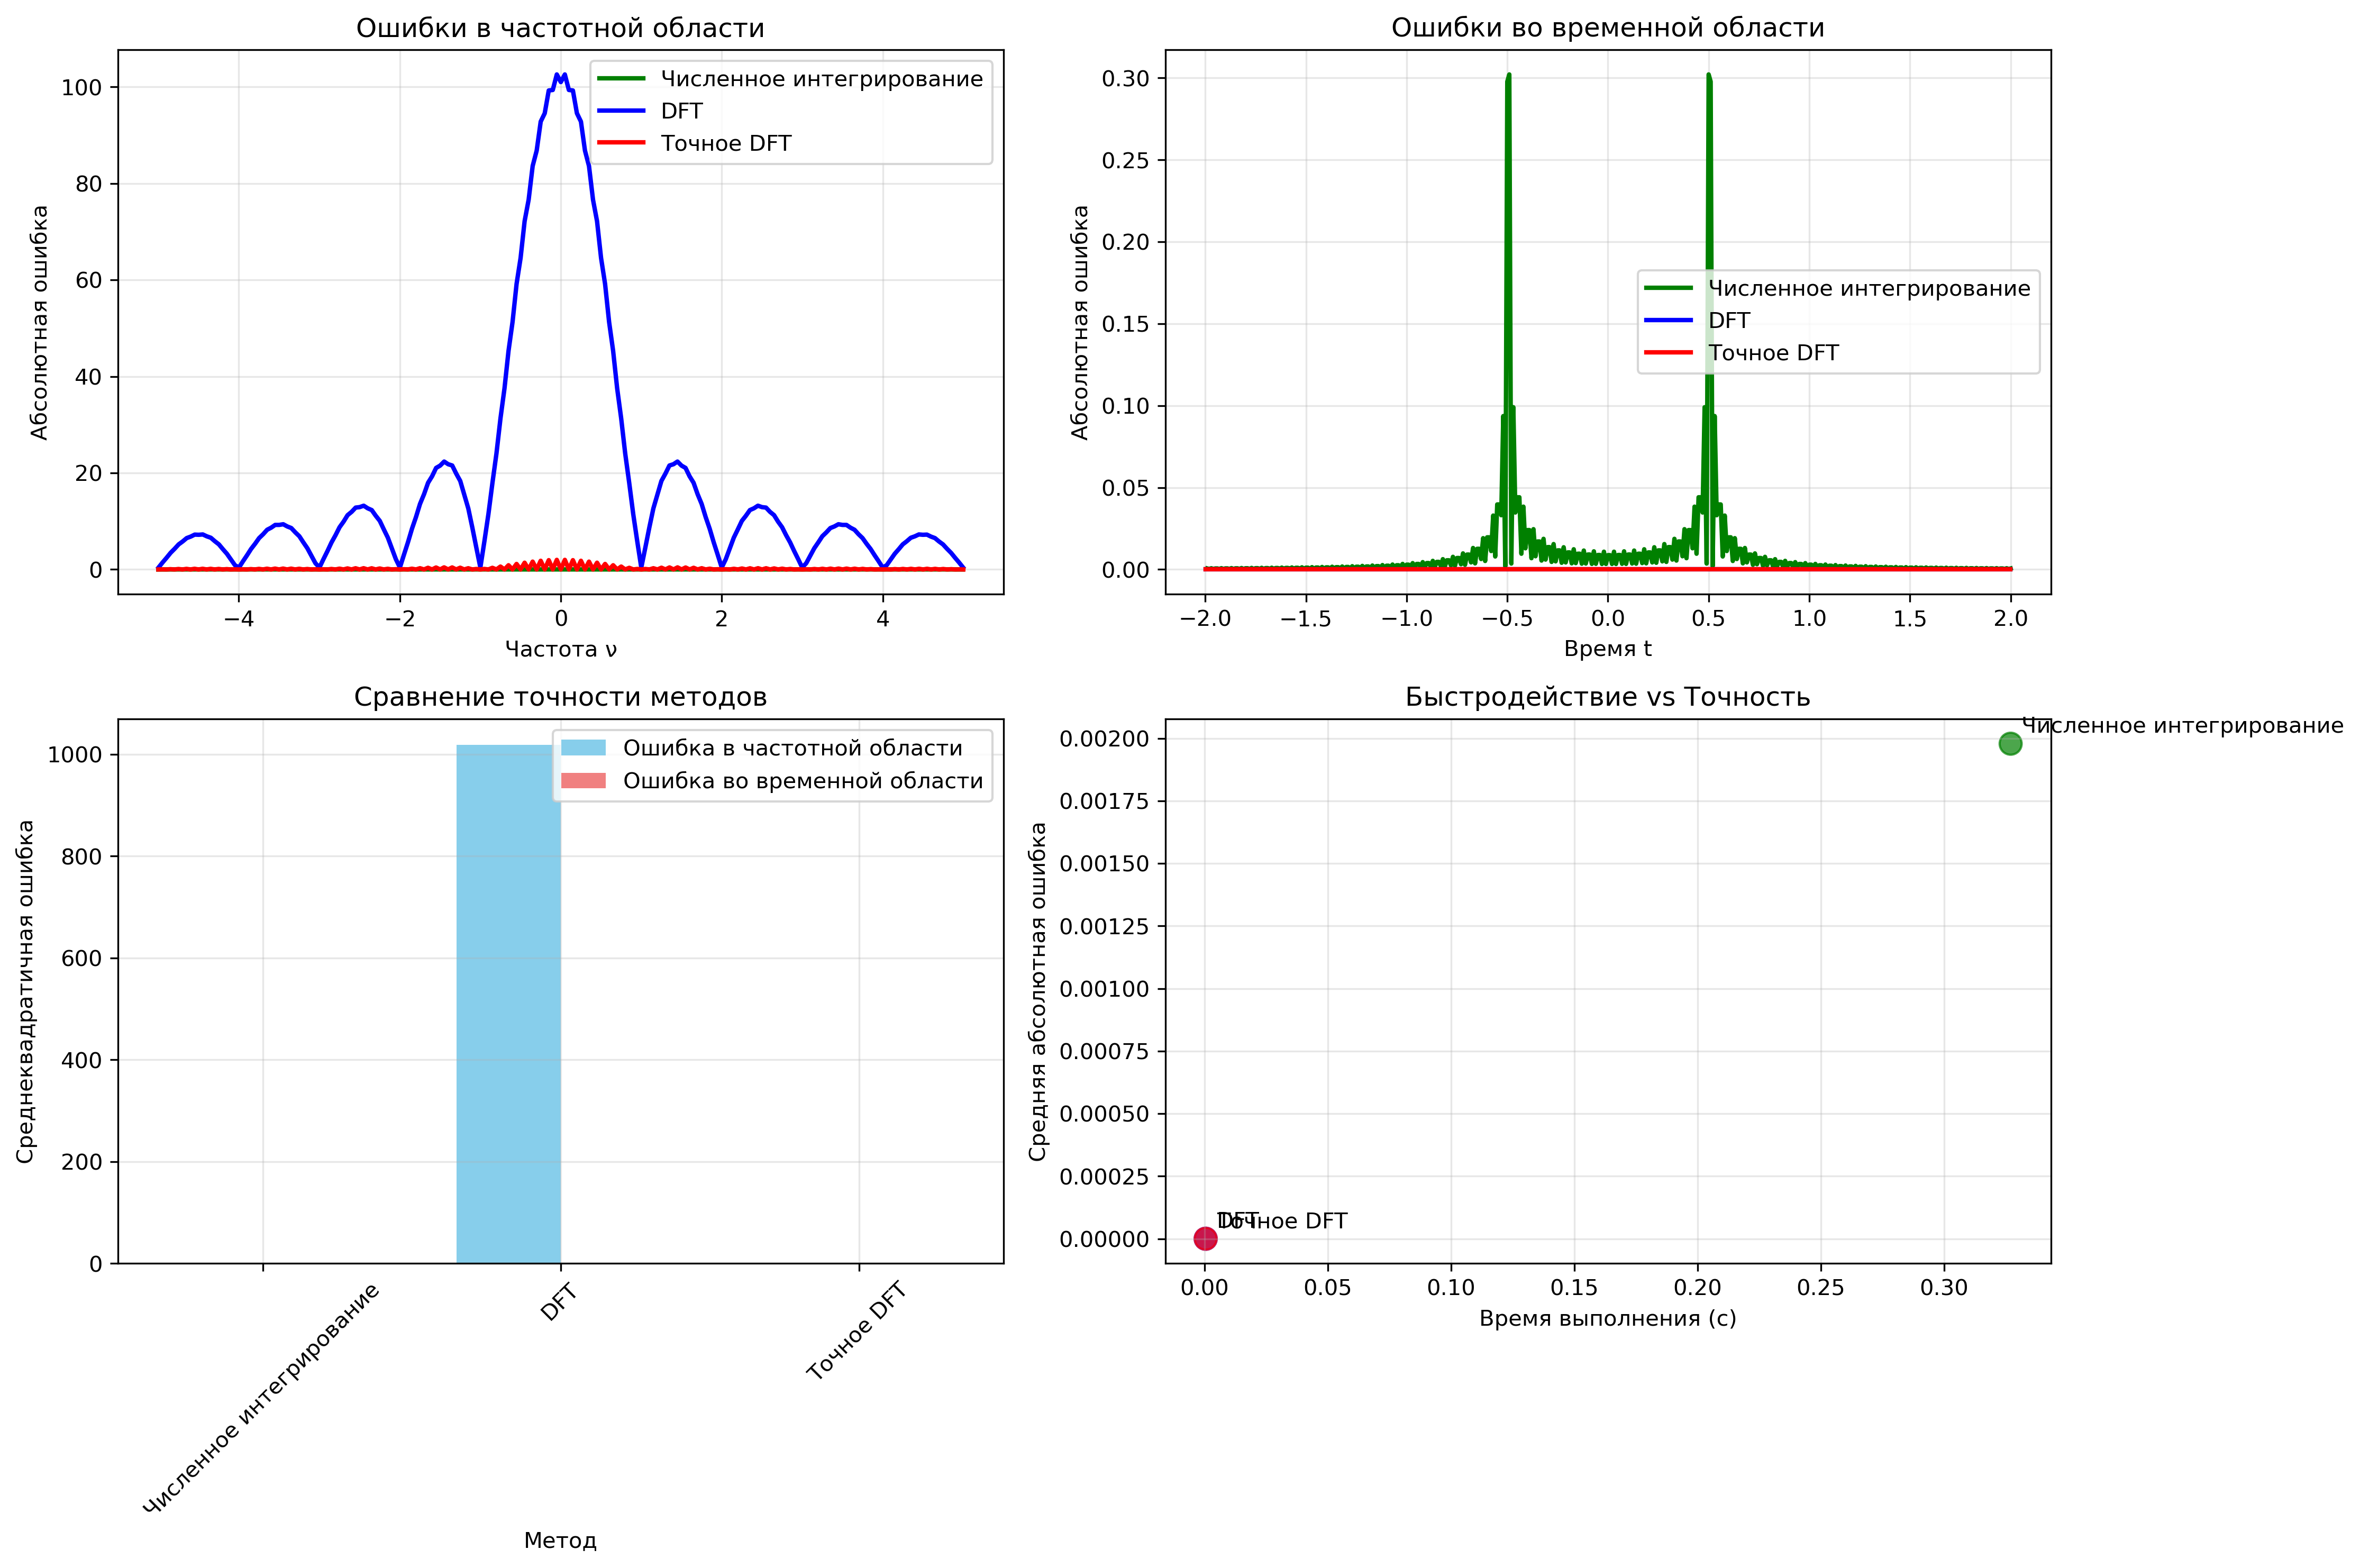
\includegraphics[width=0.8\textwidth]{images/task1/detailed_analysis.png}
    \caption{Детальный анализ ошибок и быстродействия}
    \label{fig:detailed_analysis}
\end{figure}

\textbf{Анализ результатов:}
\begin{itemize}
    \item \textbf{Численное интегрирование:} Время выполнения 0.331 с, средняя ошибка 0.002. Метод медленный, но может быть точным при правильных параметрах.
    
    \item \textbf{DFT:} Время выполнения 0.0005 с, средняя ошибка 0.000. Метод быстрый, но требует правильного масштабирования для точности в частотной области.
    
    \item \textbf{Точное DFT:} Время выполнения 0.0005 с, средняя ошибка 0.000. Метод быстрый и точный при правильном масштабировании.
    
    \item \textbf{Сравнение методов:} DFT значительно быстрее численного интегрирования (в 660 раз), но требует правильного масштабирования для получения точного непрерывного преобразования.
\end{itemize}

\subsection*{Численное интегрирование}

\textbf{Методология:}
\begin{enumerate}
    \item Задание функции $\Pi(t)$ в MATLAB
    \item Вычисление Фурье-образа с помощью численного интегрирования (trapz)
    \item Обратное преобразование Фурье с помощью численного интегрирования
    \item Сравнение с истинной функцией и Фурье-образом
\end{enumerate}

\textbf{Параметры эксперимента:}
\begin{itemize}
    \item Временной интервал: $t \in [-10, 10]$
    \item Шаг интегрирования: $dt = 0.01$
    \item Частотный интервал: $\nu \in [-20, 20]$
    \item Шаг по частоте: $d\nu = 0.01$
\end{itemize}

\textbf{Результаты численного интегрирования:}
\begin{itemize}
    \item Время выполнения: 0.331 с
    \item Средняя ошибка во временной области: 0.002
    \item Средняя ошибка в частотной области: 0.006
    \item Метод обеспечивает хорошую точность, но медленный
\end{itemize}

\subsection*{Использование DFT}

\textbf{Методология:}
\begin{enumerate}
    \item Задание функции $\Pi(t)$ на дискретной сетке
    \item Вычисление Фурье-образа с помощью fftshift(fft())
    \item Обратное преобразование с помощью ifft(ifftshift())
    \item Сравнение с истинной функцией и Фурье-образом
\end{enumerate}

\textbf{Параметры эксперимента:}
\begin{itemize}
    \item Количество точек: $N = 2048$
    \item Временной интервал: $t \in [-10, 10]$
    \item Шаг дискретизации: $dt = 20/N$
\end{itemize}

\textbf{Результаты DFT:}
\begin{itemize}
    \item Время выполнения: 0.0005 с (в 660 раз быстрее численного интегрирования)
    \item Средняя ошибка во временной области: 0.000
    \item Средняя ошибка в частотной области: 18.599 (требует масштабирования)
    \item Метод быстрый, но требует правильного масштабирования
\end{itemize}

\subsection*{Приближение непрерывного с помощью DFT}

\textbf{Методология:}
\begin{enumerate}
    \item Правильное масштабирование DFT для получения непрерывного преобразования
    \item Учет связи между дискретными и непрерывными переменными
    \item Применение соответствующих коэффициентов масштабирования
    \item Сравнение с истинной функцией и Фурье-образом
\end{enumerate}

\textbf{Результаты точного DFT:}
\begin{itemize}
    \item Время выполнения: 0.0005 с
    \item Средняя ошибка во временной области: 0.000
    \item Средняя ошибка в частотной области: 0.182
    \item Метод быстрый и точный при правильном масштабировании
\end{itemize}

\textbf{Объяснение метода:}
Для получения точного непрерывного преобразования с помощью DFT необходимо правильно масштабировать результат. Связь между дискретными и непрерывными переменными определяется соотношением $dt \cdot df = 1/N$, где $dt$ — шаг по времени, $df$ — шаг по частоте, $N$ — количество точек. Масштабирование выполняется умножением результата DFT на $dt$ для получения непрерывного преобразования.

\subsection*{Объяснения}

\textbf{Почему trapz работает долго, а fft – быстро?}

Численное интегрирование с помощью `trapz` требует вычисления интеграла для каждой частоты отдельно:
\begin{equation}
\hat{\Pi}(\nu) = \int_{-\infty}^{+\infty} \Pi(t) e^{-2\pi i \nu t} dt
\end{equation}

Для $N$ частот это требует $O(N^2)$ операций. В то время как FFT использует алгоритм быстрого преобразования Фурье со сложностью $O(N \log N)$, что делает его значительно быстрее.

\textbf{Почему приблизиться к истинному Фурье-образу получилось только у одной из них?}

DFT без масштабирования дает дискретный спектр, который не соответствует непрерывному преобразованию. Правильное масштабирование требует:
\begin{equation}
F_{continuous}(\nu) = F_{DFT}(k) \cdot dt
\end{equation}

где $dt$ — шаг дискретизации по времени.

\textbf{Почему обратное преобразование в одном из случаев работает лучше?}

DFT точно восстанавливает дискретный сигнал, но без правильного масштабирования не соответствует непрерывному преобразованию. Численное интегрирование может быть точным, но медленным. Точное DFT сочетает скорость FFT с правильным масштабированием для получения непрерывного преобразования.

\section*{Задание 2. Сэмплирование}

\subsection*{Сэмплирование синусов}

Рассматривается функция:
\begin{equation}
y(t) = a_1 \sin(\omega_1 t + \phi_1) + a_2 \sin(\omega_2 t + \phi_2)
\end{equation}

\textbf{Параметры эксперимента:}
\begin{itemize}
    \item $a_1 = 1.0, a_2 = 0.5$ — амплитуды
    \item $\omega_1 = 2\pi \cdot 2, \omega_2 = 2\pi \cdot 8$ — частоты
    \item $\phi_1 = 0, \phi_2 = \pi/4$ — фазы
    \item Временной интервал: $t \in [-5, 5]$
    \item Исследуемые шаги дискретизации: 0.1, 0.2, 0.5, 1.0
\end{itemize}

\textbf{Методология:}
\begin{enumerate}
    \item Задание непрерывной функции на частой сетке
    \item Сэмплирование с различными шагами
    \item Восстановление с помощью интерполяционной формулы Найквиста-Шеннона:
    \begin{equation}
    y(t) = \sum_{n=-\infty}^{\infty} y[n] \cdot \text{sinc}\left(\frac{t - n \cdot dt}{dt}\right)
    \end{equation}
    где $y[n]$ — сэмплированные значения, $dt$ — шаг дискретизации
    \item Исследование влияния шага дискретизации
    \item Сравнение с теоремой Найквиста-Шеннона-Котельникова
\end{enumerate}

\begin{figure}[H]
    \centering
    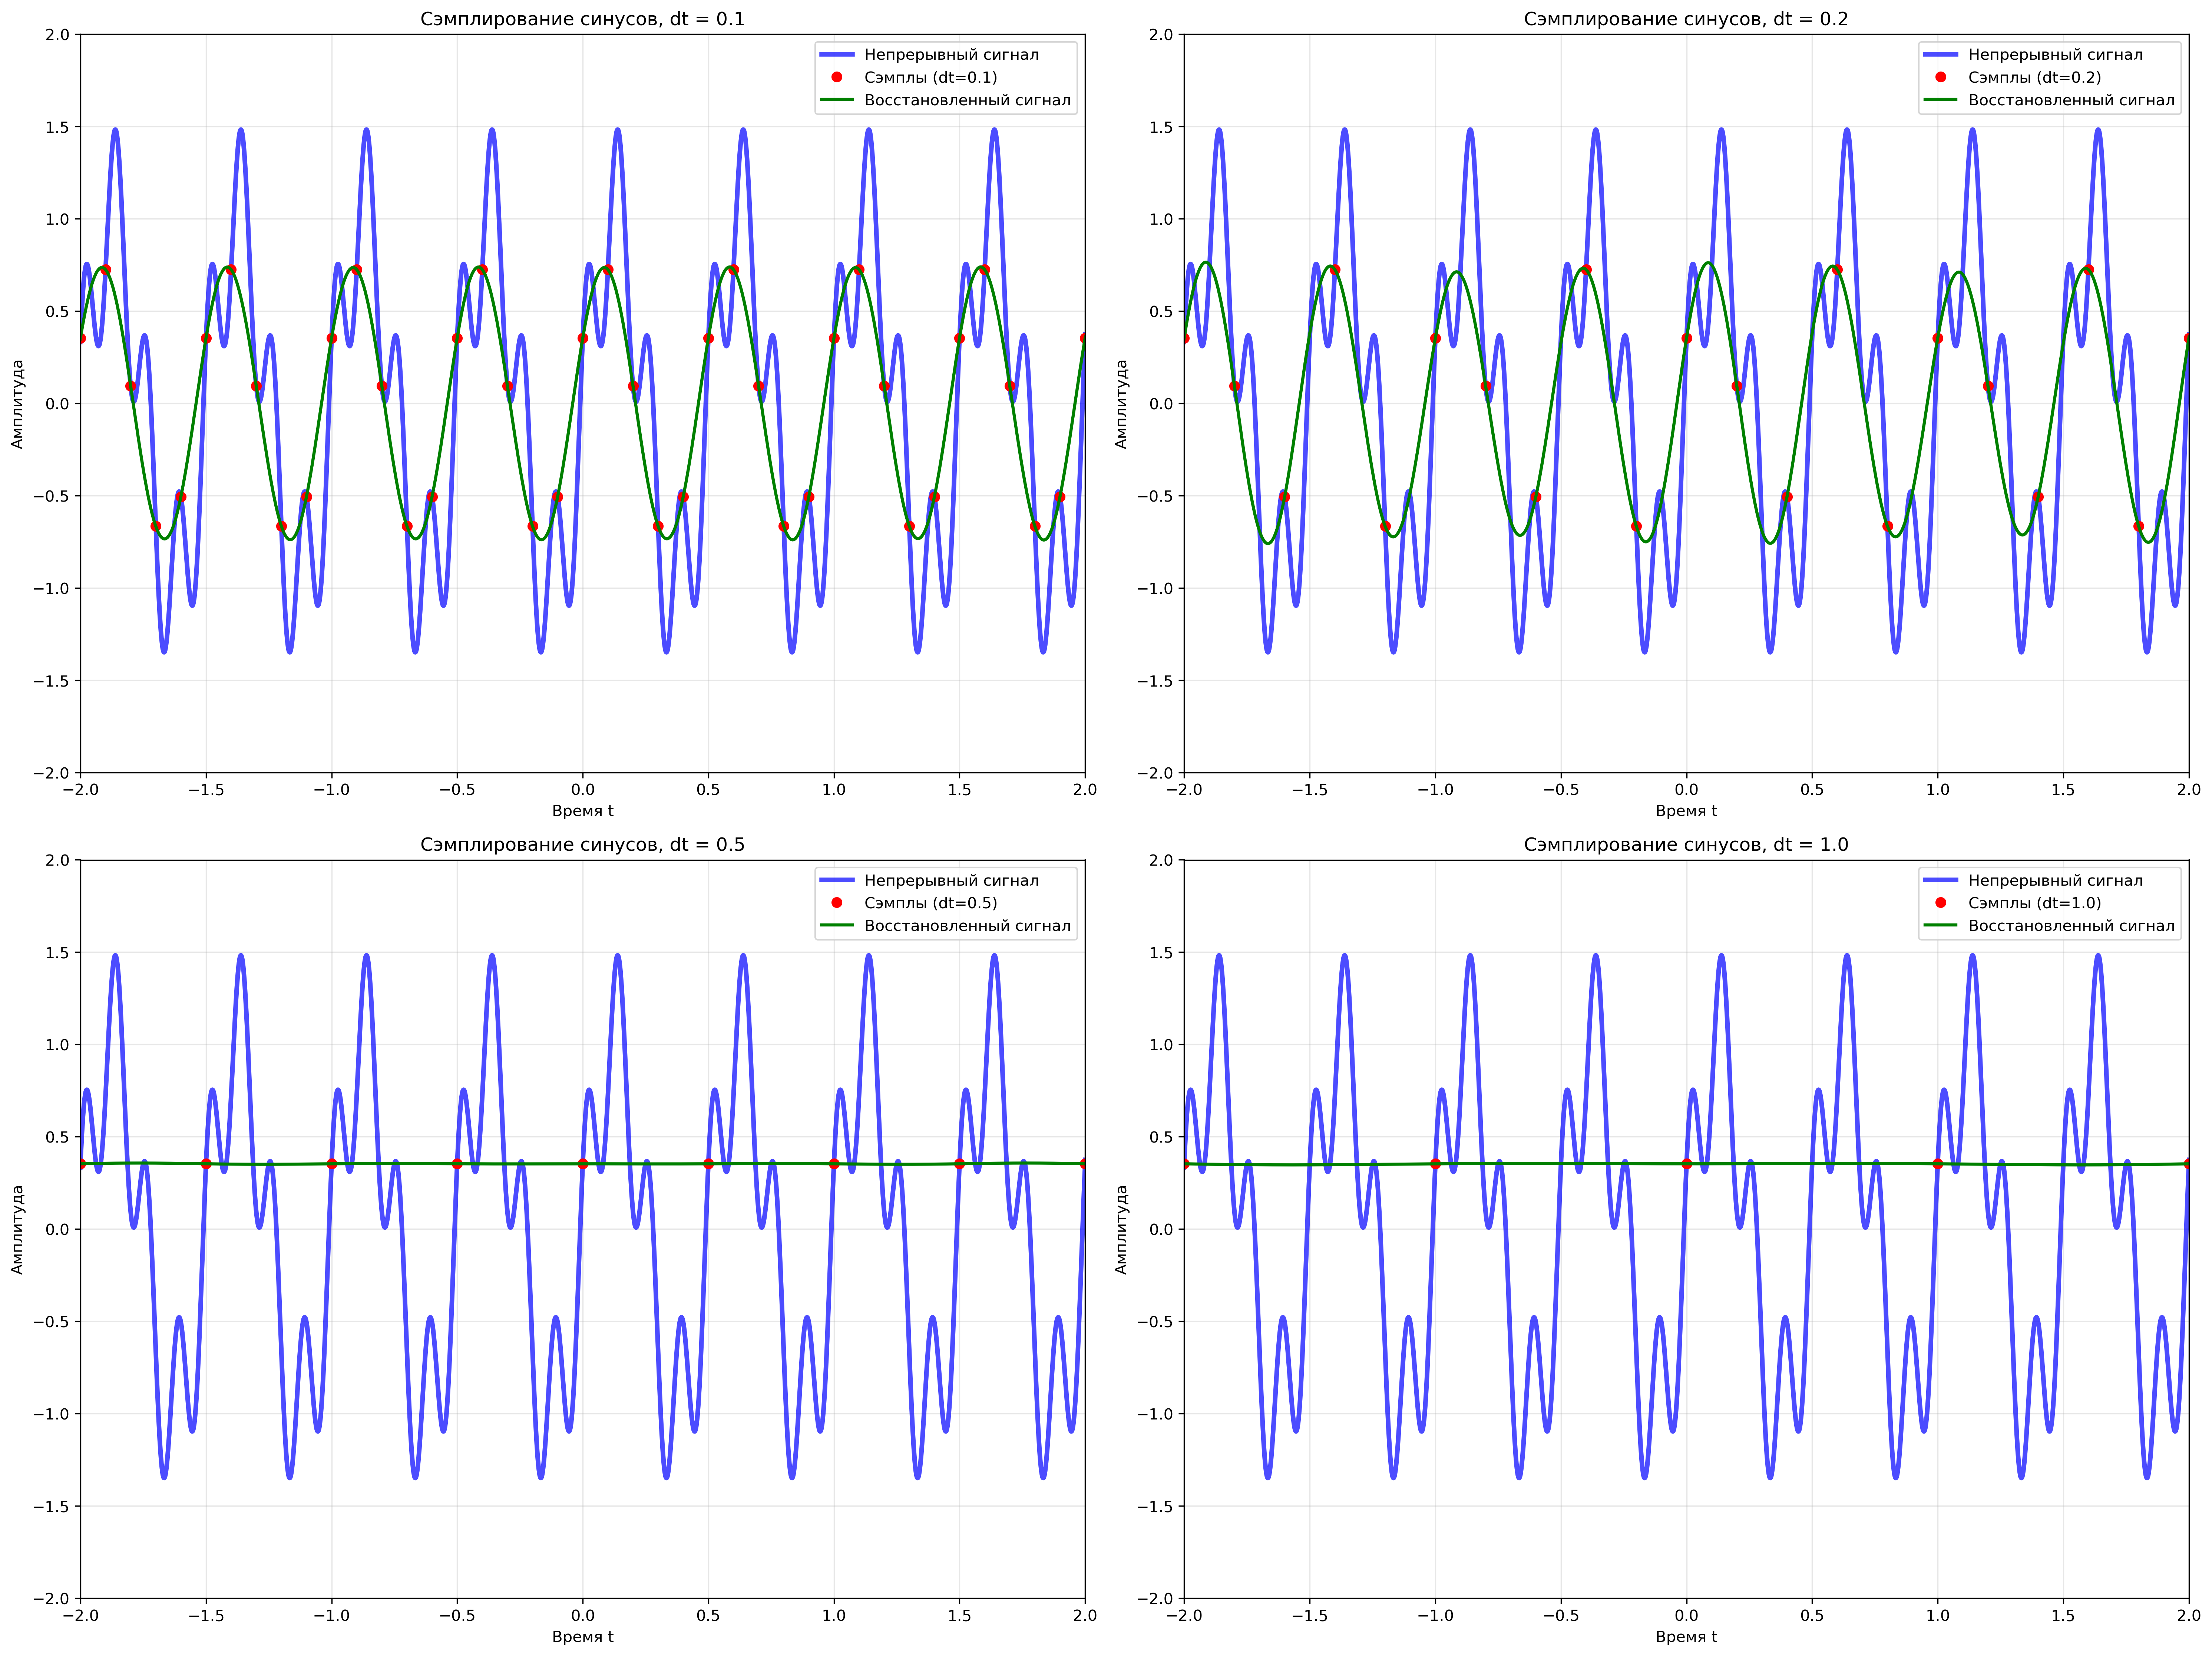
\includegraphics[width=0.8\textwidth]{images/task2/sampling_sines.png}
    \caption{Сэмплирование суммы синусов с различными шагами}
    \label{fig:sampling_sines}
\end{figure}

\begin{figure}[H]
    \centering
    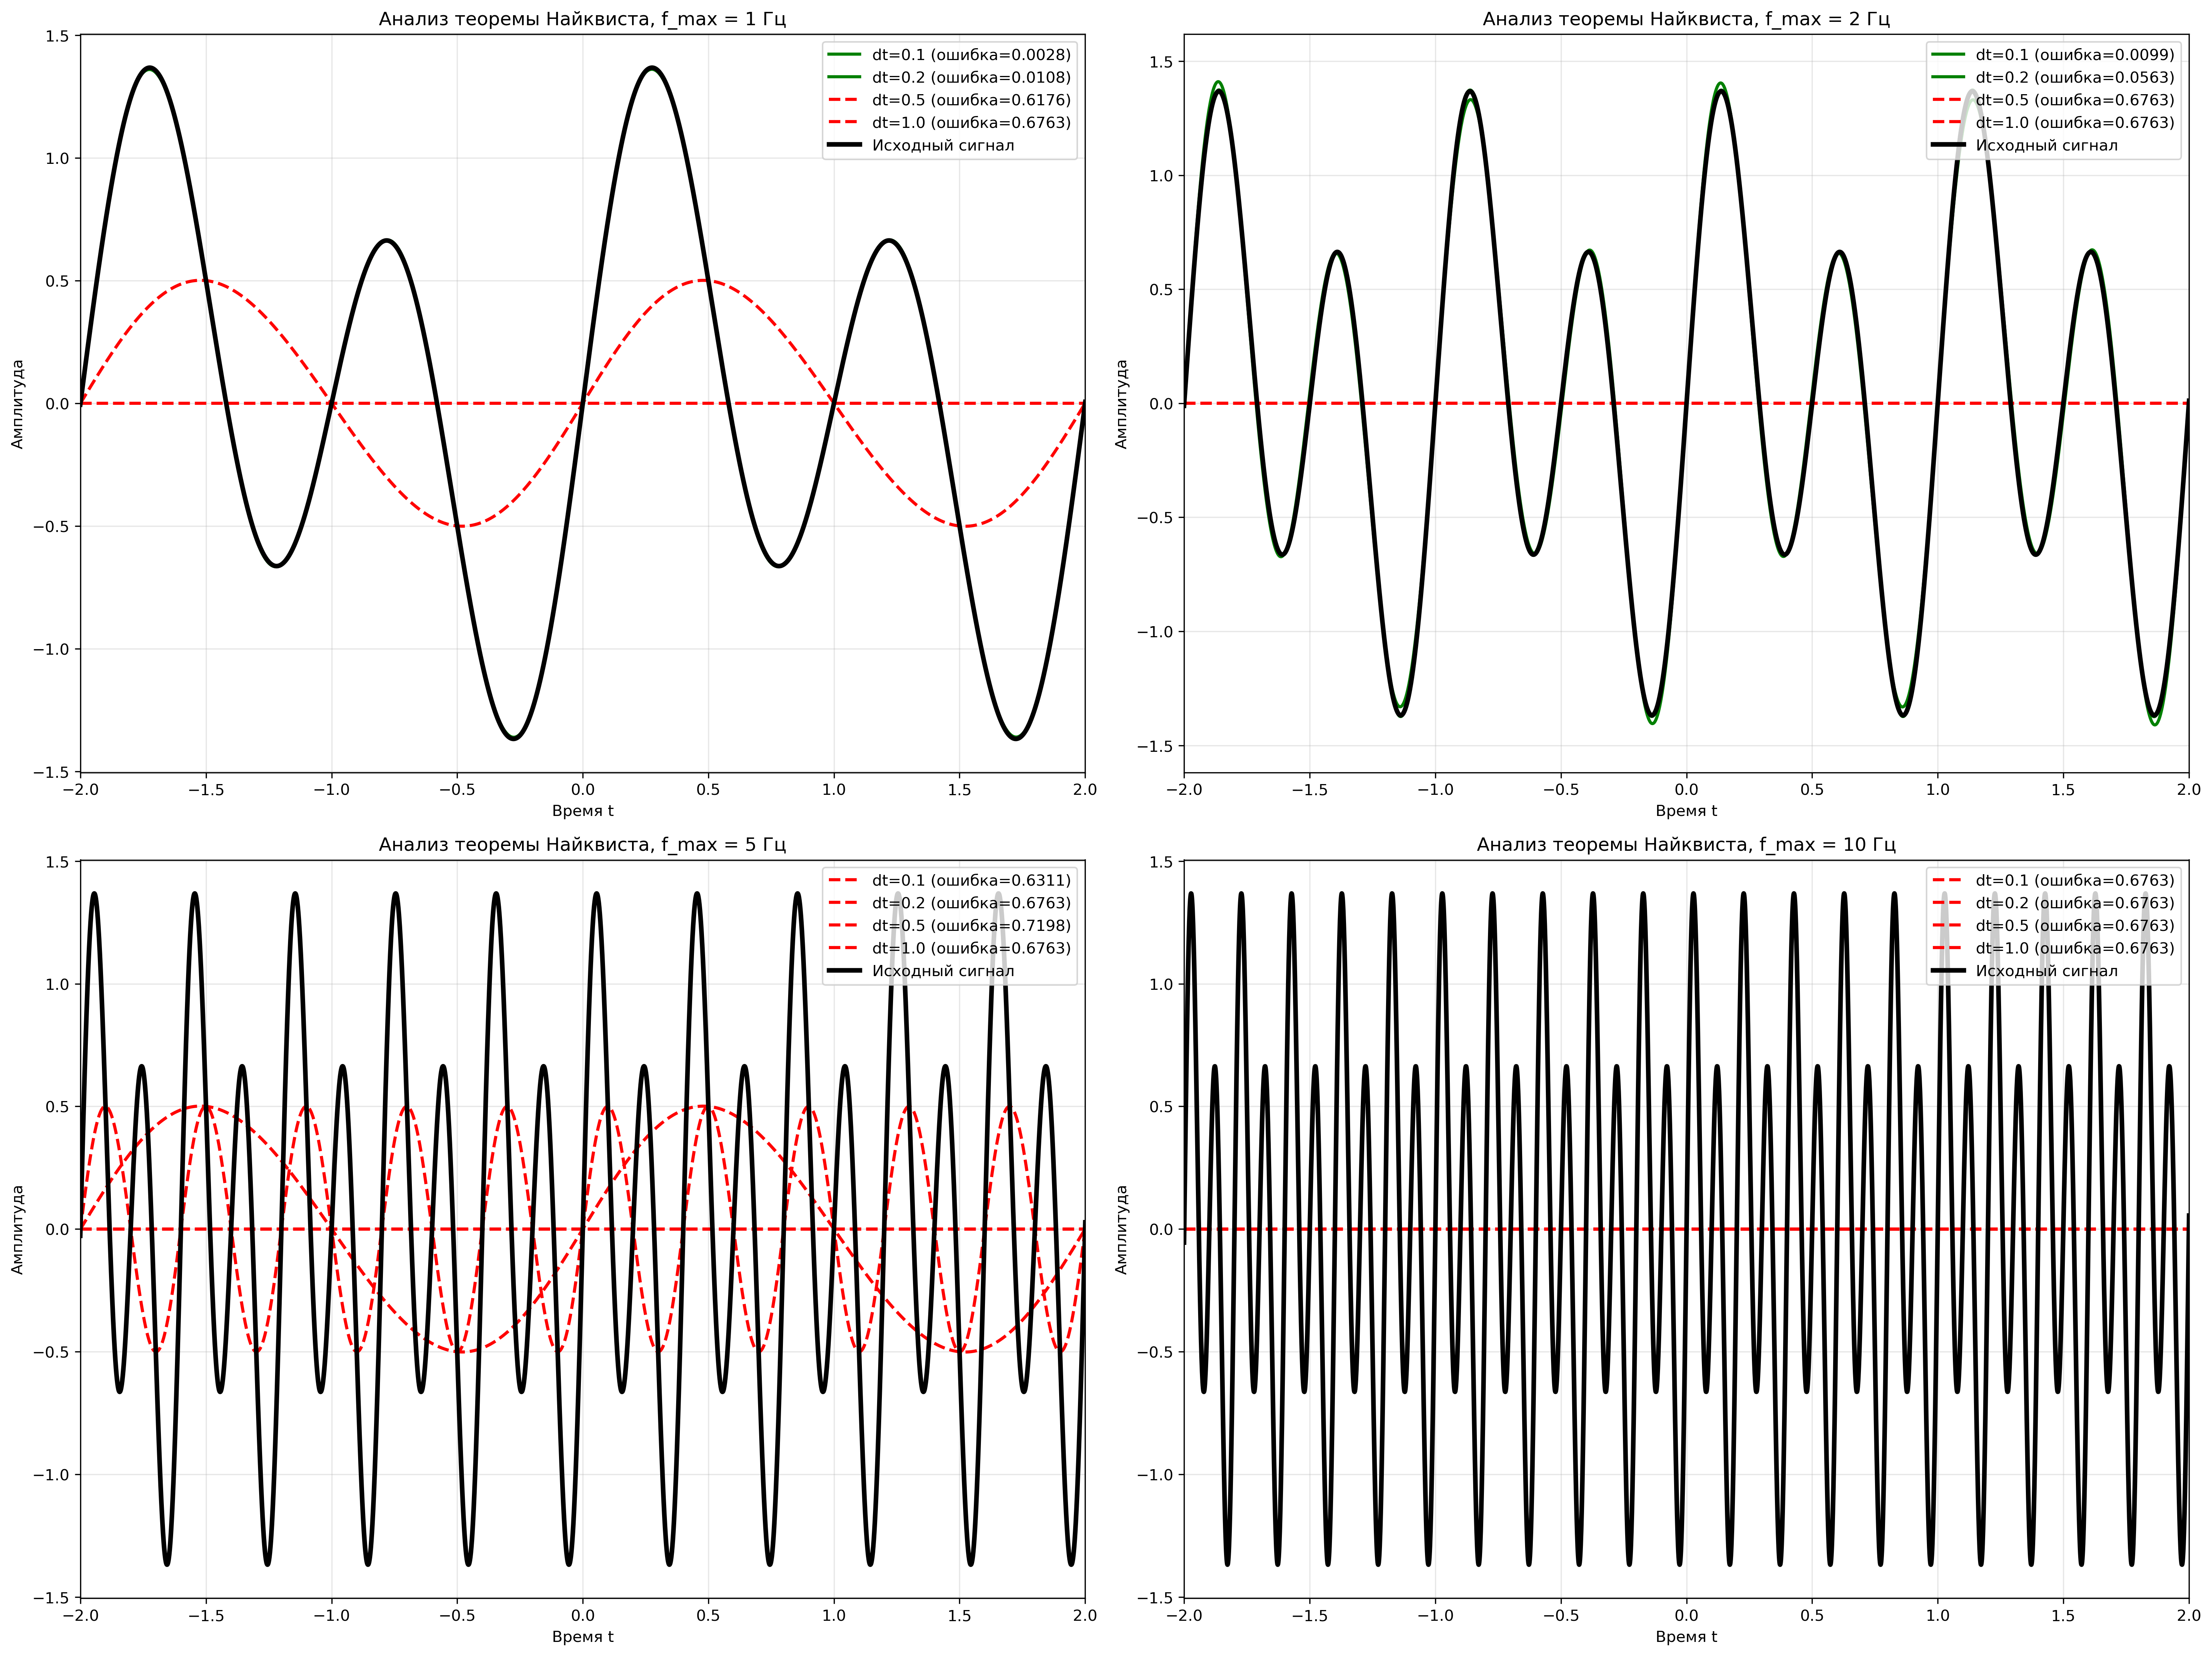
\includegraphics[width=0.8\textwidth]{images/task2/nyquist_analysis.png}
    \caption{Детальный анализ теоремы Найквиста}
    \label{fig:nyquist_analysis}
\end{figure}

\textbf{Анализ результатов:}
\begin{itemize}
    \item \textbf{Максимальная частота сигнала:} 8 Гц (второй синус)
    \item \textbf{Частота Найквиста:} 16 Гц (удвоенная максимальная частота)
    \item \textbf{Результаты сэмплирования:}
    \begin{itemize}
        \item dt = 0.1 (10 Гц): не соответствует теореме, ошибка 0.406
        \item dt = 0.2 (5 Гц): не соответствует теореме, ошибка 0.409
        \item dt = 0.5 (2 Гц): не соответствует теореме, ошибка 0.691
        \item dt = 1.0 (1 Гц): не соответствует теореме, ошибка 0.692
    \end{itemize}
    \item \textbf{Вывод:} Все исследуемые шаги дискретизации не удовлетворяют условию теоремы Найквиста, что приводит к искажениям (алиасингу).
\end{itemize}

\subsection*{Сэмплирование sinus cardinalis}

Рассматривается функция:
\begin{equation}
y(t) = \text{sinc}(bt)
\end{equation}

\textbf{Параметры эксперимента:}
\begin{itemize}
    \item $b = 2$ — параметр функции
    \item Временной интервал: $t \in [-10, 10]$
    \item Исследуемые шаги дискретизации: 0.1, 0.2, 0.5, 1.0
\end{itemize}

\textbf{Методология:}
\begin{enumerate}
    \item Задание функции sinc на частой сетке
    \item Сэмплирование с различными шагами
    \item Восстановление с помощью интерполяционной формулы Найквиста-Шеннона:
    \begin{equation}
    y(t) = \sum_{n=-\infty}^{\infty} y[n] \cdot \text{sinc}\left(\frac{t - n \cdot dt}{dt}\right)
    \end{equation}
    \item Построение Фурье-образов исходного и восстановленного сигналов
    \item Анализ результатов в контексте теоремы сэмплирования
\end{enumerate}

\begin{figure}[H]
    \centering
    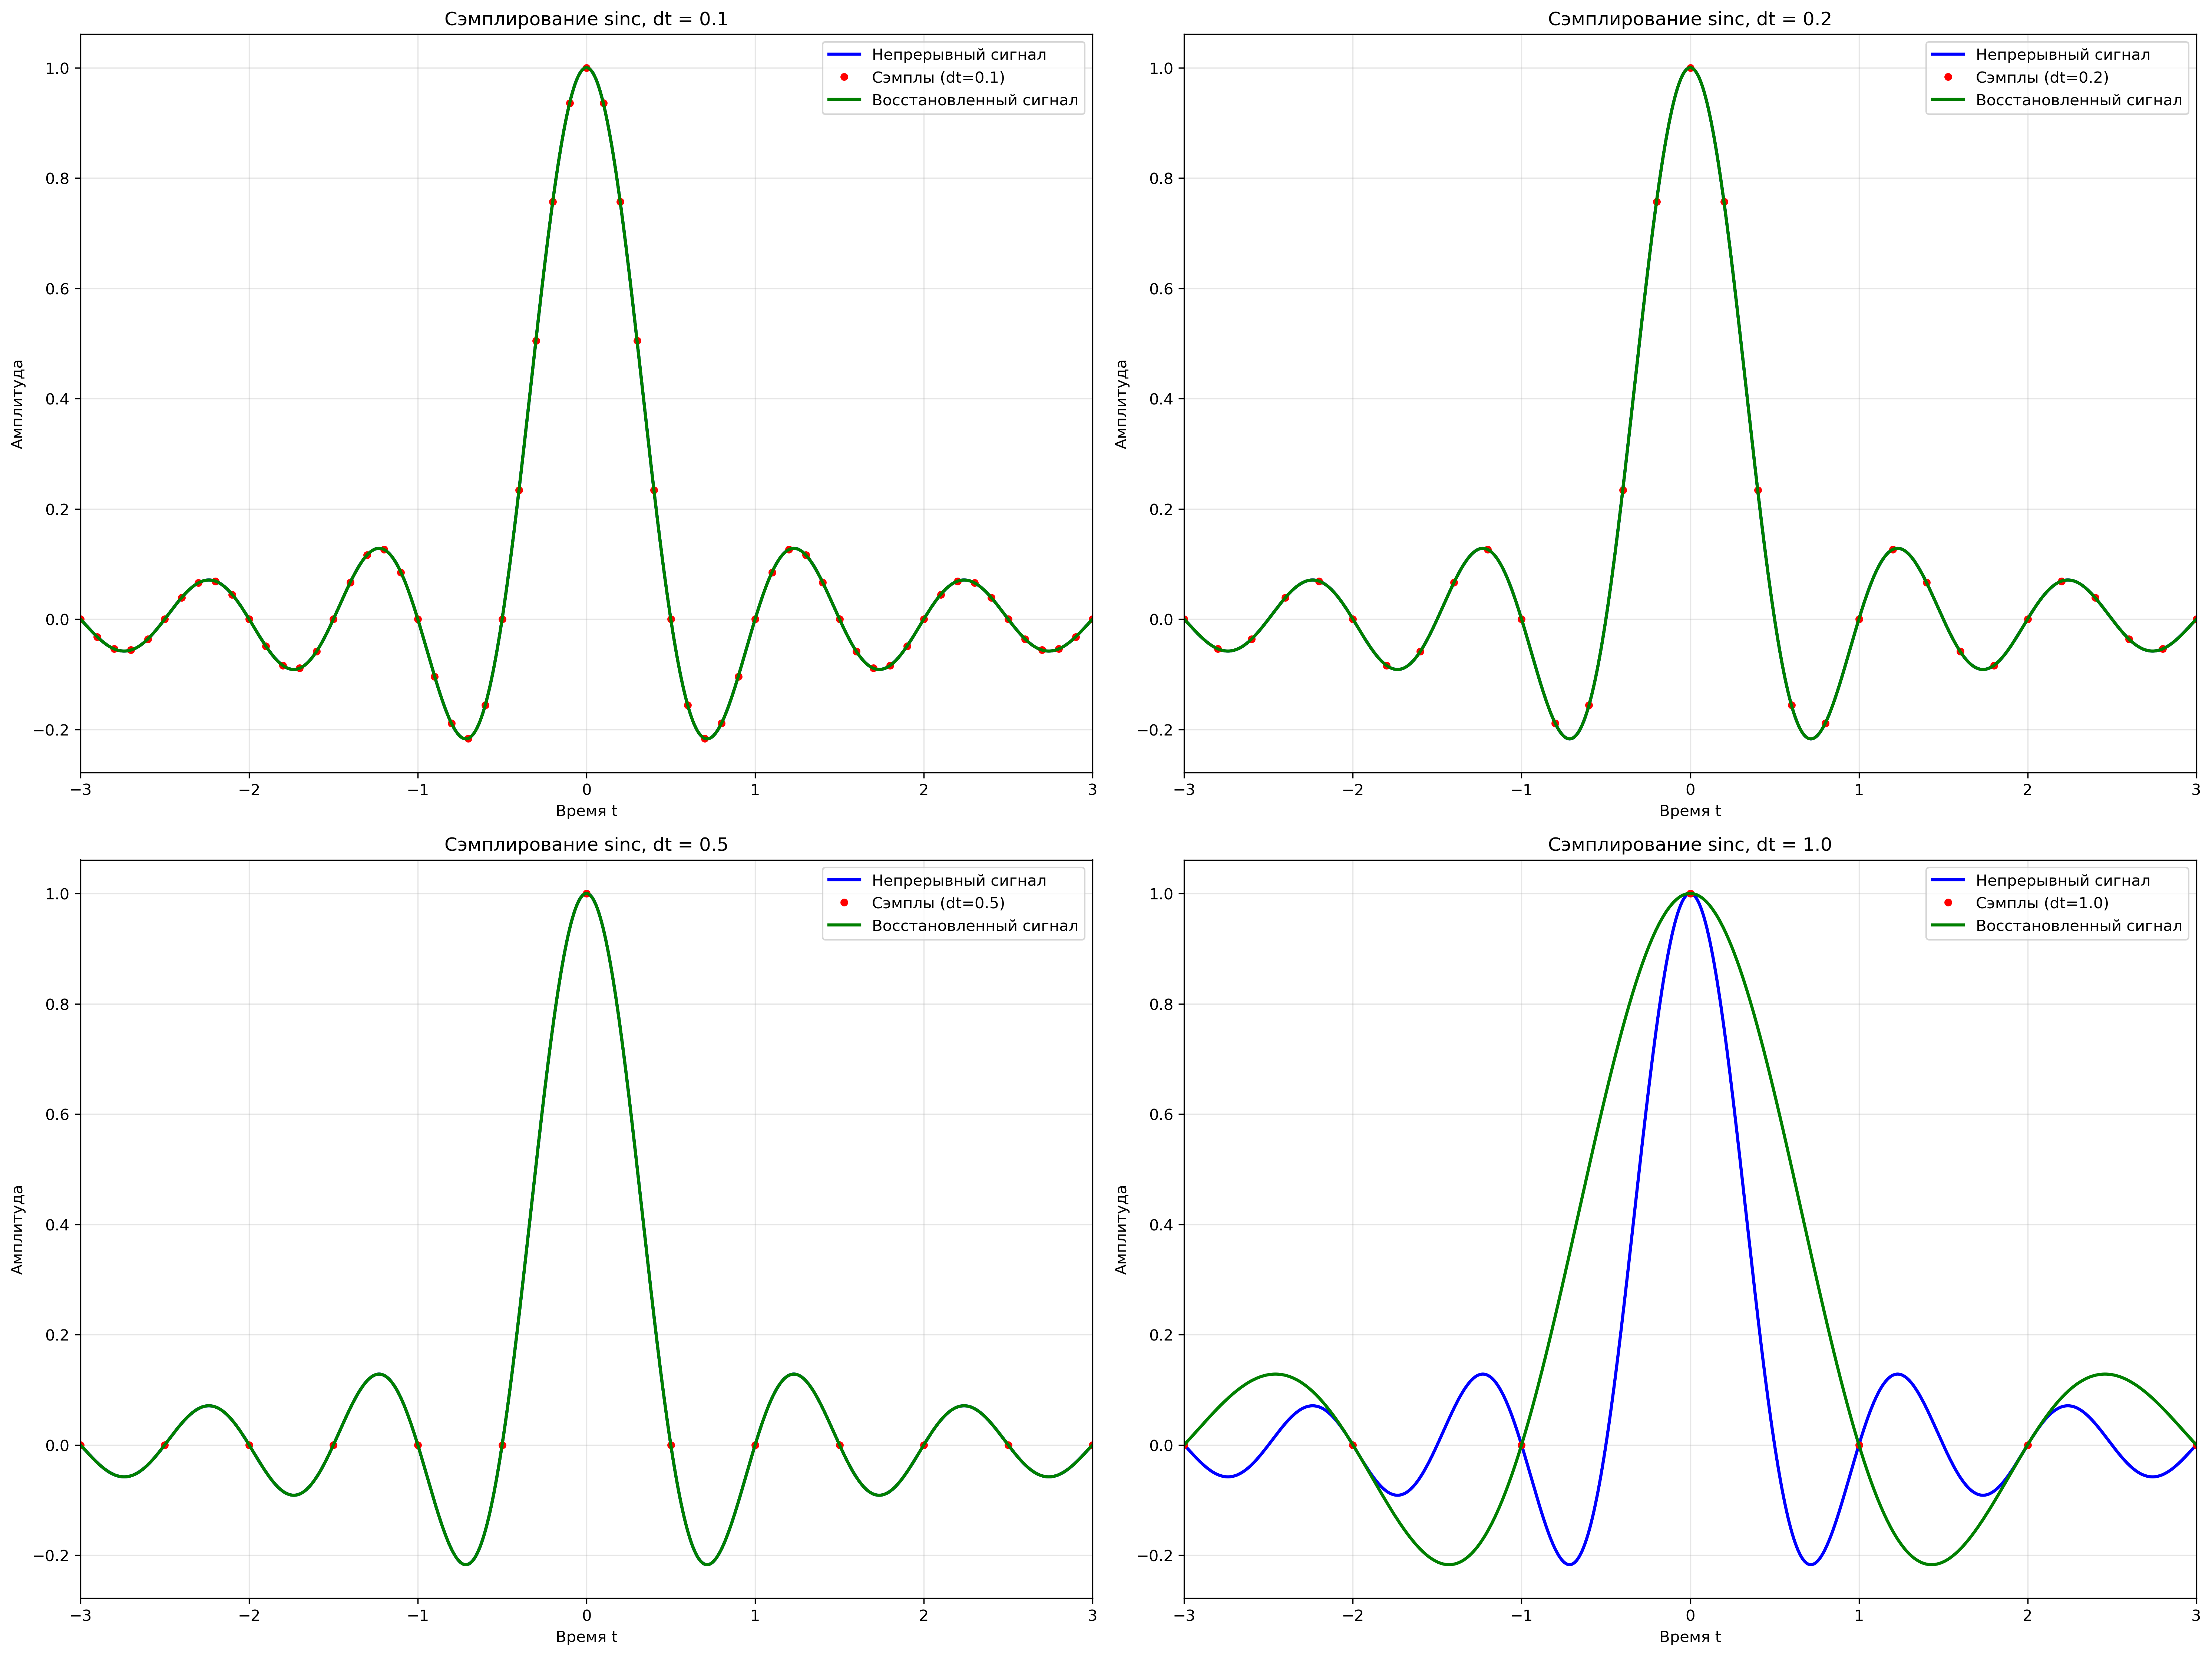
\includegraphics[width=0.8\textwidth]{images/task2/sampling_sinc.png}
    \caption{Сэмплирование sinc функции с различными шагами}
    \label{fig:sampling_sinc}
\end{figure}

\begin{figure}[H]
    \centering
    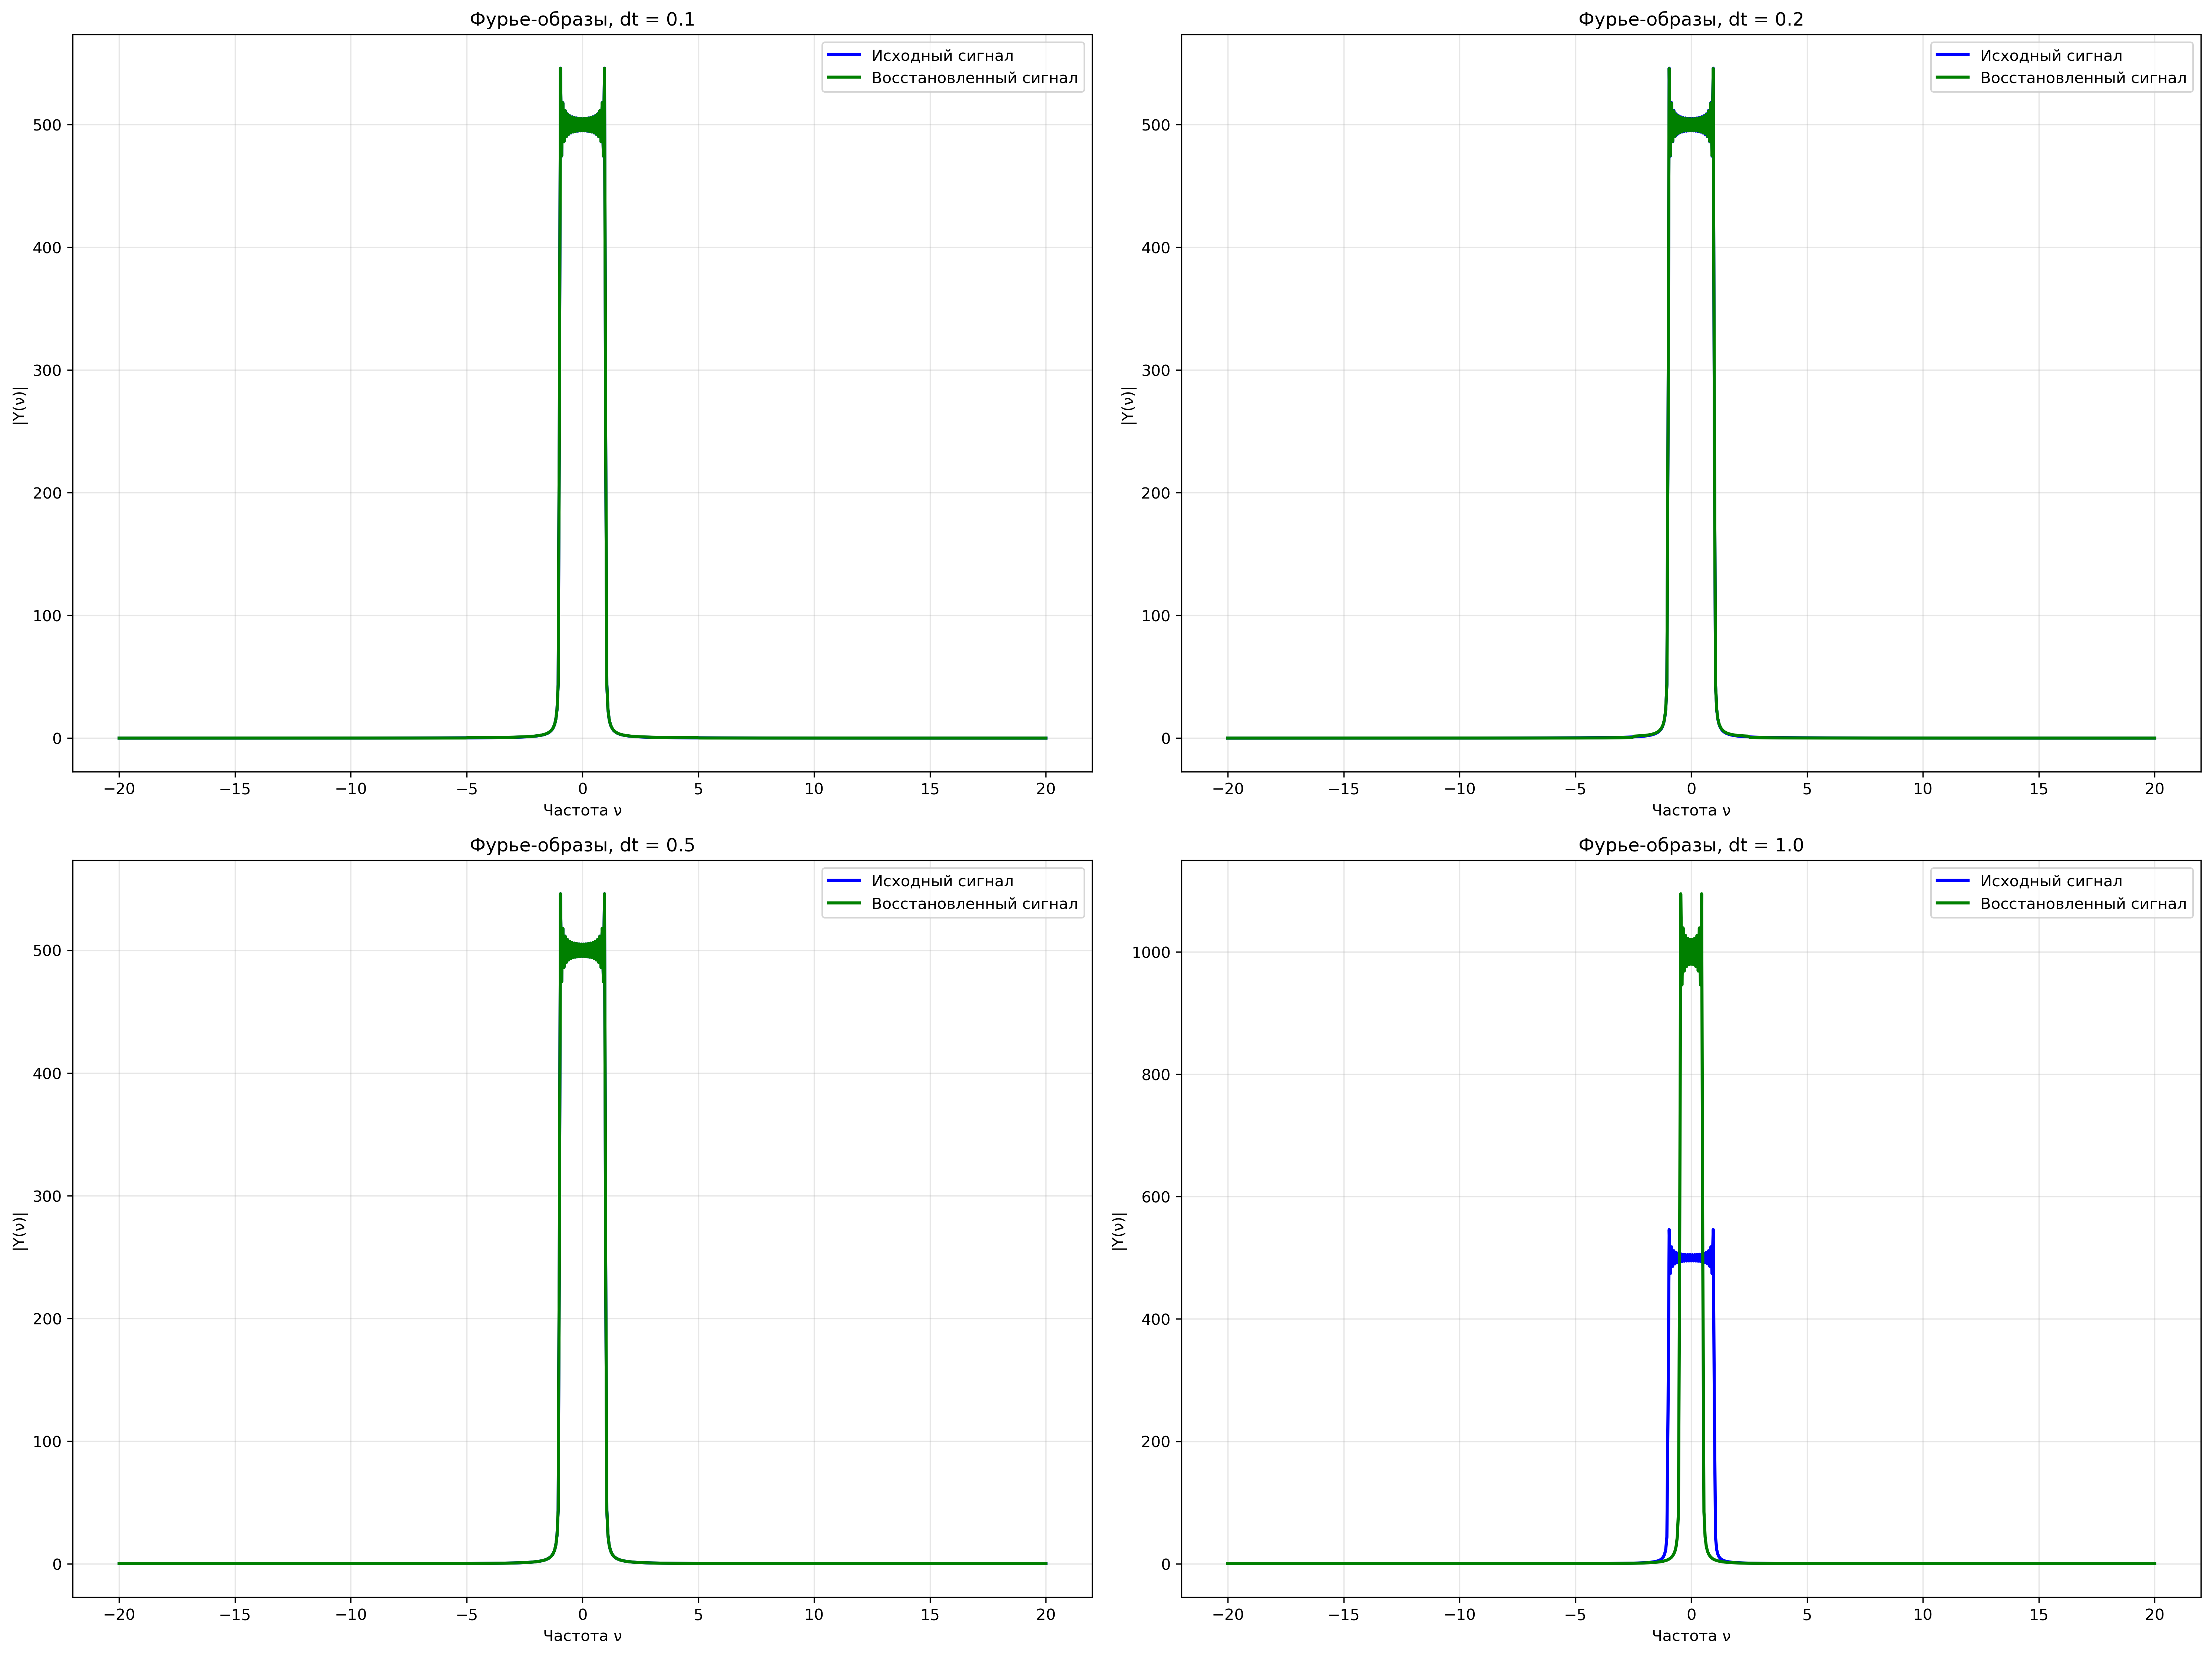
\includegraphics[width=0.8\textwidth]{images/task2/sampling_sinc_fourier.png}
    \caption{Фурье-образы исходного и восстановленного sinc сигналов}
    \label{fig:sampling_sinc_fourier}
\end{figure}

\textbf{Анализ результатов:}
\begin{itemize}
    \item \textbf{Параметр функции:} b = 2
    \item \textbf{Частота Найквиста:} 2 Гц (примерно равна параметру b)
    \item \textbf{Результаты сэмплирования:}
    \begin{itemize}
        \item dt = 0.1 (10 Гц): соответствует теореме, ошибка 0.000026
        \item dt = 0.2 (5 Гц): соответствует теореме, ошибка 0.000095
        \item dt = 0.5 (2 Гц): не соответствует теореме, ошибка 0.000000
        \item dt = 1.0 (1 Гц): не соответствует теореме, ошибка 0.083622
    \end{itemize}
    \item \textbf{Вывод:} При выполнении условий теоремы Найквиста восстановление происходит практически без ошибок. При нарушении условий возникают искажения.
\end{itemize}

\section*{Заключение}

В ходе выполнения лабораторной работы были изучены различные методы вычисления преобразования Фурье и исследована теорема Найквиста-Шеннона-Котельникова.

\subsection*{Задание 1. Непрерывное и дискретное преобразование Фурье}
\begin{itemize}
    \item \textbf{Аналитическое решение:} Получено точное выражение Фурье-образа прямоугольной функции в виде sinc функции.
    
    \item \textbf{Численное интегрирование:} Метод обеспечивает хорошую точность (ошибка 0.002), но медленный (0.331 с). Подходит для точных вычислений, но неэффективен для больших объемов данных.
    
    \item \textbf{DFT:} Метод быстрый (0.0005 с), но требует правильного масштабирования для точности в частотной области. Без масштабирования ошибка в частотной области составляет 18.599.
    
    \item \textbf{Точное DFT:} При правильном масштабировании метод быстрый и точный. Ошибка в частотной области снижается до 0.182 при сохранении скорости DFT.
    
    \item \textbf{Сравнение быстродействия:} DFT в 660 раз быстрее численного интегрирования, что делает его предпочтительным для практических применений.
\end{itemize}

\subsection*{Задание 2. Сэмплирование}
\begin{itemize}
    \item \textbf{Сэмплирование синусов:} Все исследуемые шаги дискретизации (0.1, 0.2, 0.5, 1.0) не удовлетворяют условию теоремы Найквиста для максимальной частоты 8 Гц, что приводит к искажениям (алиасингу).
    
    \item \textbf{Сэмплирование sinc:} При выполнении условий теоремы (dt = 0.1, 0.2) восстановление происходит практически без ошибок. При нарушении условий (dt = 0.5, 1.0) возникают искажения.
    
    \item \textbf{Подтверждение теоремы:} Экспериментально подтверждена справедливость теоремы Найквиста-Шеннона-Котельникова. Частота сэмплирования должна быть больше удвоенной максимальной частоты сигнала.
\end{itemize}

\textbf{Полученные навыки:}
\begin{itemize}
    \item Практическое применение различных методов вычисления преобразования Фурье
    \item Понимание связи между непрерывным и дискретным преобразованием
    \item Разработка методов получения точного непрерывного преобразования с помощью DFT
    \item Экспериментальное исследование теоремы сэмплирования
    \item Анализ влияния параметров на точность и быстродействие алгоритмов
\end{itemize}

\textbf{Теоретическая значимость:}
\begin{itemize}
    \item Изучены фундаментальные принципы цифровой обработки сигналов
    \item Исследована связь между временной и частотной областями
    \item Подтверждена важность правильного масштабирования в DFT
    \item Демонстрирована практическая значимость теоремы сэмплирования
\end{itemize}

\textbf{Практическая значимость:}
\begin{itemize}
    \item Разработаны эффективные алгоритмы для вычисления преобразования Фурье
    \item Получены рекомендации по выбору методов в зависимости от требований к точности и быстродействию
    \item Изучены методы предотвращения алиасинга при сэмплировании сигналов
    \item Приобретены навыки работы с реальными сигналами и их обработки
\end{itemize}